%%
%% This is file `sample-acmtog.tex',
%% generated with the docstrip utility.
%%
%% The original source files were:
%%
%% samples.dtx  (with options: `acmtog')
%% 
%% IMPORTANT NOTICE:
%% 
%% For the copyright see the source file.
%% 
%% Any modified versions of this file must be renamed
%% with new filenames distinct from sample-acmtog.tex.
%% 
%% For distribution of the original source see the terms
%% for copying and modification in the file samples.dtx.
%% 
%% This generated file may be distributed as long as the
%% original source files, as listed above, are part of the
%% same distribution. (The sources need not necessarily be
%% in the same archive or directory.)
%%
%% The first command in your LaTeX source must be the \documentclass command.
\documentclass[acmtog]{acmart}
%% NOTE that a single column version is required for 
%% submission and peer review. This can be done by changing
%% the \doucmentclass[...]{acmart} in this template to 
%% \documentclass[manuscript,screen]{acmart}
%% 
%% To ensure 100% compatibility, please check the white list of
%% approved LaTeX packages to be used with the Master Article Template at
%% https://www.acm.org/publications/taps/whitelist-of-latex-packages 
%% before creating your document. The white list page provides 
%% information on how to submit additional LaTeX packages for 
%% review and adoption.
%% Fonts used in the template cannot be substituted; margin 
%% adjustments are not allowed.

%%
%% \BibTeX command to typeset BibTeX logo in the docs
\usepackage{caption}
\usepackage{subcaption}

\settopmatter{printacmref=false}
\setcopyright{none}
\renewcommand\footnotetextcopyrightpermission[1]{} % removes footnote with conference information in first column

\AtBeginDocument{%
	\providecommand\BibTeX{{%
			\normalfont B\kern-0.5em{\scshape i\kern-0.25em b}\kern-0.8em\TeX}}}


%%
%% These commands are for a JOURNAL article.
\acmJournal{TOG}
\acmVolume{1}
\acmNumber{1}
\acmArticle{1}
\acmMonth{4}

%%
%% Submission ID.
%% Use this when submitting an article to a sponsored event. You'll
%% receive a unique submission ID from the organizers
%% of the event, and this ID should be used as the parameter to this command.
%%\acmSubmissionID{123-A56-BU3}

%%
%% The majority of ACM publications use numbered citations and
%% references.  The command \citestyle{authoryear} switches to the
%% "author year" style.
%%
%% If you are preparing content for an event
%% sponsored by ACM SIGGRAPH, you must use the "author year" style of
%% citations and references.
\citestyle{acmauthoryear}

%%
%% end of the preamble, start of the body of the document source.
\begin{document}
	
	%%
	%% The "title" command has an optional parameter,
	%% allowing the author to define a "short title" to be used in page headers.
	\title{Assignment 1}
	
	%%
	%% The "author" command and its associated commands are used to define
	%% the authors and their affiliations.
	%% Of note is the shared affiliation of the first two authors, and the
	%% "authornote" and "authornotemark" commands
	%% used to denote shared contribution to the research.
	
	\author{Casper Bresdahl}
	\affiliation{%
		\institution{whs715,}
		\institution{University of Copenhagen}
		\city{Copenhagen}
		\country{Denmark}}
	\email{whs715@alumni.ku.dk}
	
	%%
	%% By default, the full list of authors will be used in the page
	%% headers. Often, this list is too long, and will overlap
	%% other information printed in the page headers. This command allows
	%% the author to define a more concise list
	%% of authors' names for this purpose.
	%\renewcommand{\shortauthors}{Casper Bresdahl}
	
	%%
	%% The abstract is a short summary of the work to be presented in the
	%% article.
%	\begin{abstract}
%		Some abstract of my assignment goes here.
%	\end{abstract}
	
	\maketitle
	
	%\section{Introduction}
This week we will first introduce the theory behind advection and mean curvature flow and how we can discretize these. We will then look at the first experiment looking into how advection without any boundary issues behave compared to advection where boundaries will play a role. We will then look at the second experiment where we will compare three different boundary conditions and how these change the end result when applying mean curvature flow to a signed distance field. At the end we will conclude on our results.
	\section{Finite difference methods}
Finite difference methods are methods for solving ordinary or partial differential equations by making use of Taylor's Theorem to approximate derivatives with finite differences. This is done by discretizing the domain into a finite number of steps and then the solution of these discrete points are approximated by solving equations of finite differences. The idea can be described as replacing the derivatives by finite difference approximations. For this assignment our focus is on partial differential equations, and we will thus not discuss ordinary differential equations further. \\
We can now imagine some function partial differential equation$f(x,y)$. If we discretize \textit{f} we sample a finite number of values along both the \textit{x} and \textit{y} axis and we denote this spacing by respectively $\Delta x$ and $\Delta y$. If we keep the spatial information of sampling \textit{f} every $\Delta x$ and $\Delta y$ unit in mind, we can think of this discretization as constructing a computational grid, or just grid for short, where each node in the grid is a functional value. Increasing the sampling rate, i.e decreasing $\Delta x$ and $\Delta y$, results in a larger and finer grid but also in a better approximation to \textit{f}, whereas decreasing the sampling rate results in a smaller and coarser grid. The 'area' in which we sample is called the domain, and the partial differential equation, in our case \textit{f}, which defines what happens in the domain is called a governing equation. With our grid we now have a notion of 'neighbours' and we can now look at how to approximate the derivatives of our grid by finite differences derived from Taylor's Theorem.

\subsection{Forward, backward and central difference approximations}
Assuming the function whose derivatives are to be approximated is properly behave we can construct a Taylor series:
\begin{equation*}
	f(x_i + \Delta x) = f(x_i) + \frac{f^{(1)}(x_i)}{1!}\Delta x + \frac{f^{(2)}(x_i)}{2!}\Delta x^2 + \dots + \frac{f^{(n)}(x_i)}{n!}\Delta x^n + \mathbf{o}(\Delta x)
\end{equation*}
It is this series we will use to construct finite difference approximations. If we wish to compute $\frac{\partial f}{\partial x}$ we use a first order Taylor expansion, that is, we use the above Taylor series, but truncate it after the first derivative:
\begin{equation}
	f(x_i + \Delta x) = f(x_i) + \frac{f^{(1)}(x_i)}{1!}\Delta x + \mathbf{o}(\Delta x) \label{eq:1}
\end{equation}
Using \autoref{eq:1} we can now solve for the first derivative:
\begin{align*}
	f(x_i + \Delta x) &= f(x_i) + \frac{f^{(1)}(x_i)}{1!}\Delta x + \mathbf{o}(\Delta x) \iff\\
	\frac{f(x_i + \Delta x)}{\Delta x} &= \frac{f(x_i)}{\Delta x} + f^{(1)}(x_i) + \frac{\mathbf{o}(\Delta x)}{\Delta x} \iff\\
	f^{(1)}(x_i) &= \frac{f(x_i + \Delta x)}{\Delta x} - \frac{f(x_i)}{\Delta x} - \frac{\mathbf{o}(\Delta x)}{\Delta x} 
\end{align*}
If we now disregard $- \frac{\mathbf{o}(\Delta x)}{\Delta x}$ we get an approximation known as the \textit{forward difference approximation}:
\begin{equation*}
	\frac{\partial}{\partial x}f(x_i) \approx \frac{f(x_i + \Delta x) - f(x_i)}{\Delta x}
\end{equation*}
Similarly we can write the first order Taylor expansion as:
\begin{equation}
	f(x_i - \Delta x) = f(x_i) - \frac{f^{(1)}(x_i)}{1!}\Delta x + \mathbf{o}(\Delta x) \label{eq:2}
\end{equation}
Using \autoref{eq:2} we can solve for the first derivative:
\begin{align*}
	f(x_i - \Delta x) &= f(x_i) - \frac{f^{(1)}(x_i)}{1!}\Delta x + \mathbf{o}(\Delta x) \iff\\
	\frac{f(x_i - \Delta x)}{\Delta x} &= \frac{f(x_i)}{\Delta x} - f^{(1)}(x_i) + \frac{\mathbf{o}(\Delta x)}{\Delta x} \iff\\
	f^{(1)}(x_i) &= \frac{f(x_i)}{\Delta x} - \frac{f(x_i - \Delta x)}{\Delta x} + \frac{\mathbf{o}(\Delta x)}{\Delta x} 
\end{align*}
If we now disregard $\frac{\mathbf{o}(\Delta x)}{\Delta x}$ we get an approximation known as the \textit{backward difference approximation}:
\begin{equation*}
	\frac{\partial}{\partial x}f(x_i) \approx \frac{f(x_i) - f(x_i - \Delta x)}{\Delta x}
\end{equation*}
We can now also add the forward difference approximation and the backward difference approximation together:
\begin{align}
	2\frac{\partial}{\partial x}f(x_i) &\approx \frac{f(x_i + \Delta x) - f(x_i)}{\Delta x} + \frac{f(x_i) - f(x_i - \Delta x)}{\Delta x} \iff\\
	\frac{\partial}{\partial x}f(x_i) & \approx \frac{1}{2}\frac{f(x_i + \Delta x) - f(x_i) + f(x_i) - f(x_i - \Delta x)}{\Delta x} \iff \\
	\frac{\partial}{\partial x}f(x_i) & \approx \frac{f(x_i + \Delta x) - f(x_i - \Delta x)}{2\Delta x} \label{eq:3}
\end{align}
\autoref{eq:3} is known as the \textit{central difference approximation}.

\subsection{Higher order and higher dimensions approximations}
We now turn our attention to higher order derivatives. If we want to compute $\frac{\partial^2 f}{\partial x^2}$ we can use the central difference approximation recursively, and use mid points to evaluate the finite differences:
\begin{align*}
	\frac{\partial^2}{\partial x^2}f(x_i) &\approx \frac{\frac{\partial}{\partial x}f(x_i + \frac{1}{2}\Delta x) - \frac{\partial}{\partial x}f(x_i - \frac{1}{2}\Delta x)}{\Delta x}\\
	& = \frac{\frac{f(x_i + \Delta x) - f(x_i)}{\Delta x} - \frac{f(x_i) - f(x_i - \Delta x)}{\Delta x}}{\Delta x}\\
	& =  \frac{f(x_i + \Delta x) - 2f(x_i) + f(x_i - \Delta x)}{\Delta x^2}
\end{align*}

For higher dimensions we get more or less the same expressions with the notation slightly changed. Taking the central difference approximation gives us:
\begin{align*}
	\frac{\partial f(x_i,y_j)}{\partial x} &\approx \frac{f(x_i+\Delta x,y_j) - f(x_i-\Delta x,y_j)}{2\Delta x}\\
	\frac{\partial f(x_i,y_j)}{\partial y} &\approx \frac{f(x_i,y_j +\Delta y) - f(x_i,y_j -\Delta y)}{2\Delta y}
\end{align*}
We can also combine the higher order and higher dimensions to find:
\begin{align*}
	\frac{\partial^2}{\partial y \partial x} f_{i,j} &= \frac{\partial}{\partial x}\left(\frac{\partial}{\partial y}f_{i,j}\right)\\
	&\approx \frac{\partial}{\partial x}\left( \frac{f_{i,j +1} - f_{i,j -1}}{2\Delta y} \right)\\
	&\approx \frac{f_{i+1,j+1} - f_{i-1,j+1} - f_{i+1,j-1} + f_{i-1,j-1}}{4\Delta x \Delta y}
\end{align*}
Where we here shorten the notation and have $f_{i,j} = f(x_i,y_j)$ and $f_{i+1,j+1} = f(x_i + \Delta x,y_j + \Delta y)$.
	\section{Toy example}
We can now look at the toy example from the notebook and slides. We define $u(x,y): \mathbb{R}^2 \rightarrow \mathbb{R}$ and we define the partial differential equation:
\begin{equation}
	f(x,y) = \nabla^2 u - \kappa^2 u = \frac{\partial^2 u}{\partial x^2} + \frac{\partial^2 u}{\partial y^2} + \kappa^2 u \label{eq:4}
\end{equation}
Where \textit{f} is known to us. As \textit{u} is unknown we need a way to simplify the partial derivatives in \autoref{eq:4}. This is where our finite difference approximations comes into the picture. Using (for instance) the central difference approximation we can now approximate the partial derivatives in terms of the surrounding nodes in our sampled grid. Using central difference approximation we can thus simplify \autoref{eq:4} to:
\begin{align*}
	f_{i,j} &= \frac{u_{i+1,j} - 2u_{i,j} + u_{i-1,j}}{\Delta x^2} + \frac{u_{i,j+1} - 2u_{i,j} + u_{i,j-1}}{\Delta y^2} - \kappa^2 u\\
	&= \frac{1}{\Delta x^2}u_{i-1,j} + \frac{1}{\Delta y^2}u_{i,j-1} + \left(-\kappa^2 - \frac{2}{\Delta x^2} - \frac{2}{\Delta y^2}\right)u_{i,j} \\
	&\quad + \frac{1}{\Delta y^2}u_{i,j+1} + \frac{1}{\Delta x^2}u_{i+1,j}
\end{align*}
If we now substitute all the coefficients before the \textit{u} terms with $c's$ (to shorten / generalize notation) we can derive \textit{update formulas} for the \textit{u} terms. We can for instance derive the update formula for the unknown $u_{i,j}$ as:
\begin{equation*}
	u_{i,j} = \frac{f_{i,k} - c_{i-1,j}u_{i-1,j} - c_{i,j-1}u_{i,j-1} - c_{i,j+1}u_{i,j+1} - c_{i+1,j}u_{i+1,j}}{c_{i,j}}
\end{equation*}
We here refer to \textit{f} as the \textit{source term}. From the update formula of $u_{i,j}$ we see which other \textit{u} terms $u_{i,j}$ depends on. We can visualize this in terms of a \textit{stencil} which more visually gives a notion of which other nodes in our grid our nodes depend on.
\begin{figure}[H]
	\centering
	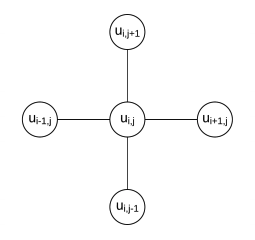
\includegraphics[width=0.4\linewidth]{Materials/stencil}
	\caption{Visualization of a stencil. Illustration taken from lecture slides.}
	\label{stencil}
\end{figure}
In \autoref{stencil} we can see an illustration of a stencil. We can imagine running this stencil over each node in our grid, which would then gives us the update formula for each node in the grid in terms of dependent nodes. However, we quickly realize that the stencil would stick outside our grid at the boundaries. We thus need some boundary conditions to handle what should happen at the boundaries. 

\subsection{Boundaries}
\begin{figure}[H]
	\centering
	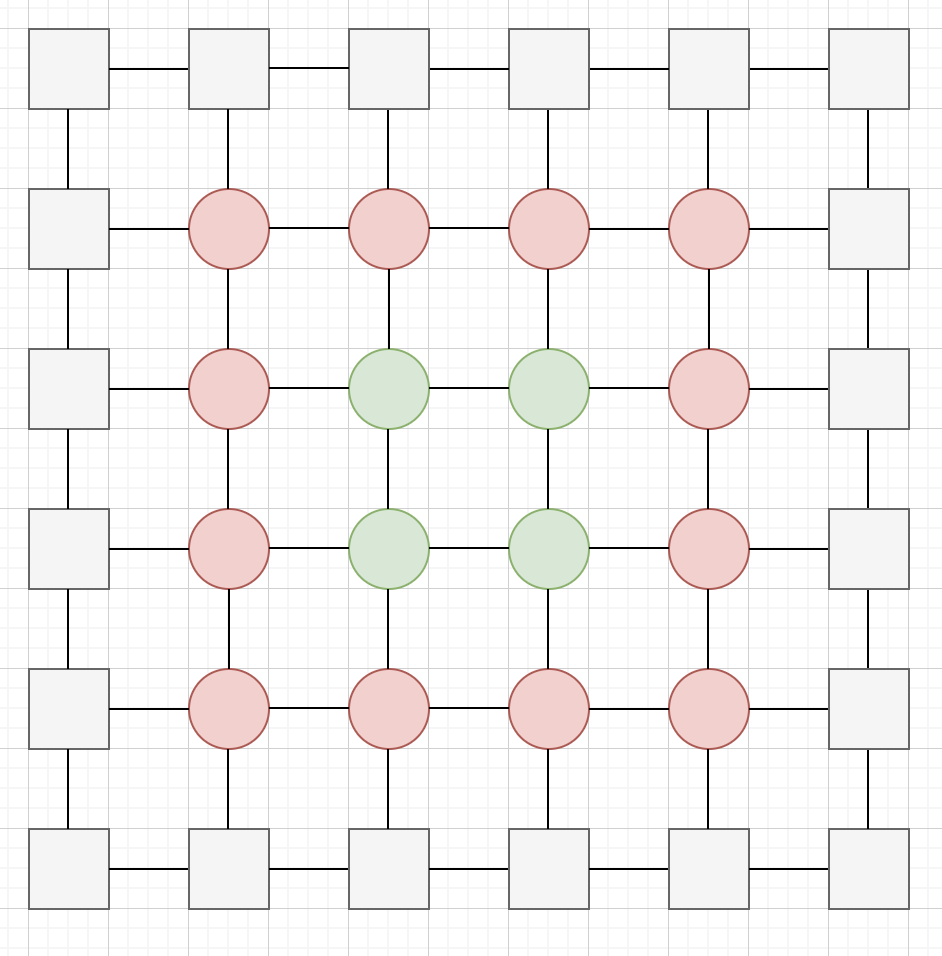
\includegraphics[width=0.3\linewidth]{Materials/grid}
	\caption{Visualization of a grid with the green and red circles being domain nodes, red circles being boundary nodes and the square nodes being ghost nodes..}
	\label{grid}
\end{figure}
Two common boundary conditions are Dirichlet and von Neumann boundary conditions. We define them as:
\begin{align*}
	u(x,y) &= k_d, \quad \forall x,y \in \Gamma\\
	\frac{\partial u}{\partial x} &= k_n, \quad \forall x,y \in \Gamma
\end{align*}
Where $\Gamma$ is the 'boundary of the boundary nodes' (the boundary nodes can be seen in \autoref{grid}). We can apply one of two techniques to deal with boundary conditions, we either use elimination of unknown variables or we use ghost nodes. If we choose to apply a von Neumann boundary condition and we choose to apply elimination of variables to handle it, then for the left side of the grid, using central difference approximations, we will have:
\begin{align*}
	\frac{\partial^2 u_{1,j}}{\partial x^2} &= \frac{\frac{\partial}{\partial x}u_{\frac{1}{2},j} - \frac{u_{2,j} - u_{1,j}}{\Delta x}}{\Delta x}\\
	&= \frac{u_{1,j} - u_{2,j}}{\Delta x^2}
\end{align*}
As $\frac{\partial}{\partial x}u_{\frac{1}{2},j}$ is zero according to the von Neumann boundary condition. That is, we can compute the left boundary conditions as a negative forward difference approximation. Similarly, if $x_i = 5$ is our right boundary we have for the right boundary conditions:
\begin{align*}
	\frac{\partial^2 u_{5,j}}{\partial x^2} &= \frac{\frac{u_{5,j} - u_{4,j}}{\Delta x} - \frac{\partial}{\partial x}u_{5\frac{1}{2},j}}{\Delta x}\\
	&= \frac{u_{5,j} - u_{4,j}}{\Delta x^2}
\end{align*}
Which is a backwards difference approximation. This also extends symmetrically to the top and bottom boundary conditions.\\
If we choose to use the ghost node approach we then extends our grid. This can be seen in \autoref{grid} where the circles is our domain and the squares are 'extra' nodes which we append to ensure the stencil never goes out of bounds. To find the values of these ghost nodes we can now 'unpack' the von Neumann boundary conditions from above:
\begin{equation*}
	\frac{\partial}{\partial x}u_{\frac{1}{2},j} = \frac{u_{1,j} - u_{o,j}}{\Delta x} = 0
\end{equation*}
This implies $u_{0,j} = u_{1,j}$ (we would obtain similar results if we looked at the other boundaries), that is our boundaries should 'reflect' or mirror the domain values it is 'facing'. 

\subsection{Solutions}
Now that we have dealt with our boundaries, we can compute solutions in two different ways. First we can use our stencil, and iteratively go over all domain nodes in our grid updating each node according to our update formula. This requires we make an initial guess for the values of our nodes which simply could be all of them are equal to zero at iteration zero. We would keep updating our nodes until they 'converge', i.e. the nodes no longer change.\\
Another way to compute a solution is to note the stencils form linear systems of equations where we have:
\begin{align*}
	f_{1,1} &= c_{1,0}u_{1,0} + c_{0,1}u_{0,1} + c_{1,1}u_{1,1} + c_{2,1}u_{2,1} + c_{1,2}u_{1,2}\\
	&\vdots \\
	f_{n-1,m-1} & = c_{n-1,m-2}u_{n-1,m-2} + c_{n-2,m-1}u_{n-2,m-1}\\
	&\quad + c_{n-1,m-1}u_{n-1,m-1} + c_{n,m-1}u_{n,m-1} + c_{n-1,m}u_{n-1,m}
\end{align*}
Where \textit{n} and \textit{m} are the size of the grid. We can similarly write a linear system for the boundary conditions. If we split the coefficients and the \textit{u} values we can construct the matrix system $\mathbf{Au} = \mathbf{f}$ where \textbf{A} encodes the coefficients and \textbf{f} is our vectorized grid values. We can compute the vector index from the 2d grid indices as $k = jN+i$ where \textit{N} is the number of columns in the grid. To construct \textbf{A} we similarly use the encoding $\mathbf{A}_{(jN+i),(bN+a)} = c_{a,b}$ where we would define \textit{a} and \textit{b} in relation to \textit{i} and \textit{j}, i.e. if we want to encode the middle node of our stencil, this would have index $\mathbf{A}_{jN+i),jN+i)}$ and the left arm of the stencil would have index $\mathbf{A}_{jN+i),((j-1)N+i)}$. This maps our stencils to rows of \textbf{A} as seen in \autoref{stencilencoding}. After the encoding we can simply solve $\mathbf{Au} = \mathbf{f}$ for \textbf{u}. This process is called \textit{matrix assembly}.
\begin{figure}[H]
	\centering
	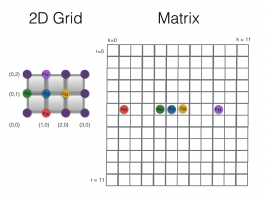
\includegraphics[width=0.5\linewidth]{Materials/stencilencoding}
	\caption{Visualization of a grid with the green and red circles being domain nodes, red circles being boundary nodes and the square nodes being ghost nodes.}
	\label{stencilencoding}
\end{figure}
	\section{Experiments}
As a first experiment we can experiment with what happens when we change the values of \textit{f}, i.e. our grid values, and when we change $\kappa$ in our toy example. In the notebook we define $f = X+Y$ where \textit{X} and \textit{Y} are linear sequences of numbers. This defines a flat grid with a 'tilt'. If we now define $f = X^4+Y^4$ the grid is no longer linear but instead gets curved as illustrated in \autoref{e1}. If we increase the value of $\kappa$ we make the denominator in the update formula for $u_{i,j}$ smaller which results in $u_{i,j}$ increasing. If the grid is linear, we see this change simply 'shifts' the grid up, \autoref{e4}, whereas if the grid is non-linear we get more curve to the solution and the shift, \autoref{e2}. We can also change the von Neumann boundary condition such that the constant becomes 1. The results of this is the boundary of the solution becoming very steep as seen in \autoref{e3}.
\begin{figure}[H]
	\centering
	\begin{subfigure}[b]{0.45\linewidth}
		\centering
		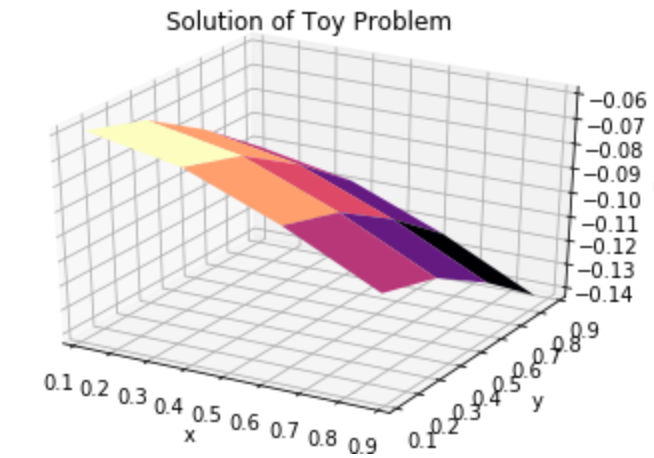
\includegraphics[width=\linewidth]{Materials/f4}
		\caption{Solution when the grid $f = X^4+Y^4$.}
		\label{e1}
	\end{subfigure}
	\hfill
	\begin{subfigure}[b]{0.45\linewidth}
		\centering
		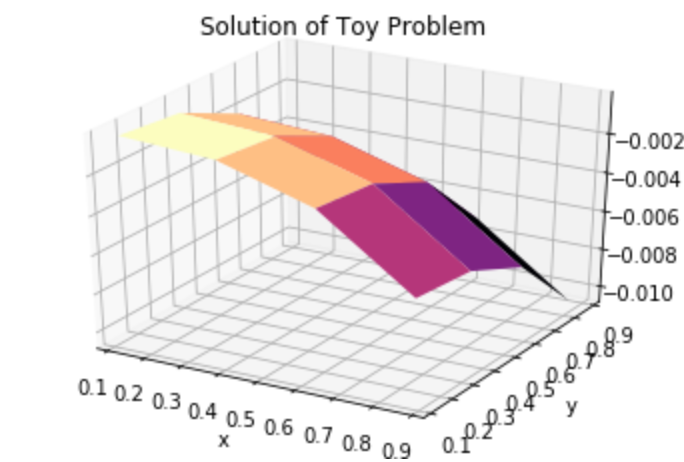
\includegraphics[width=\linewidth]{Materials/f4k10}
		\caption{Solution when the grid $f = X^4+Y^4$ and $\kappa = 10$.} 
		\label{e2}
	\end{subfigure}
	\begin{subfigure}[b]{0.45\linewidth}
		\centering
		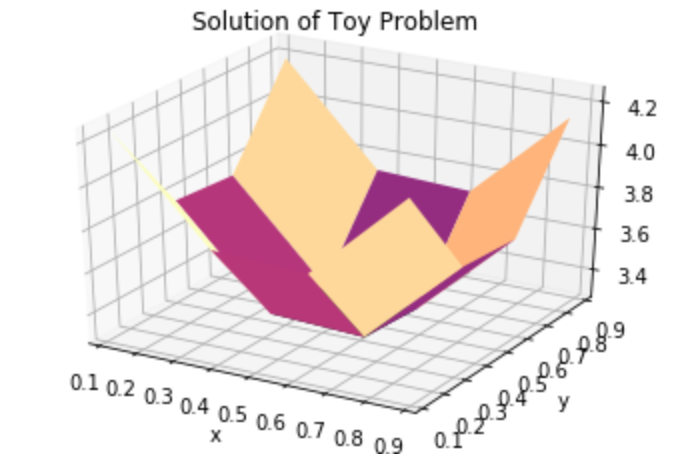
\includegraphics[width=\linewidth]{Materials/b=1}
		\caption{Solution when the grid $f = X+Y$, $\kappa = 2$ and von Neumann conditions equal 1.} 
		\label{e3}
	\end{subfigure}
	\hfill
	\begin{subfigure}[b]{0.45\linewidth}
		\centering
		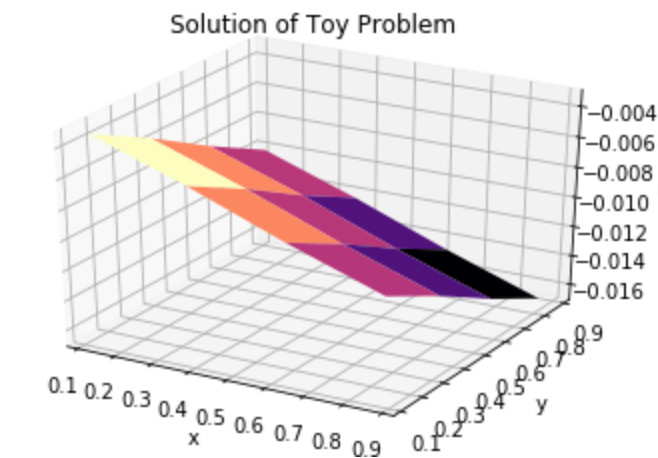
\includegraphics[width=\linewidth]{Materials/k10}
		\caption{Solution when the grid $f = X+Y$ and $\kappa = 10$.\\\hfill} 
		\label{e4}
	\end{subfigure}
\end{figure} 
As another experiment, we can look at the time it takes to solve $\mathbf{Au} = \mathbf{f}$ for bigger and bigger square grids. We can do this by doing the matrix assembly and then time how long it takes numpy to perform \textit{np.linalg.solve}. We do this over 10 iteration where we solve the same system and then take the average of the times to avoid some of the variance of how many resources the computer has available at the time of the computation. In \autoref{runtime} we see that the time to solve the linear system grows exponentially as we increase the grid size. This is not entirely surprising as the number of grid cells in a square grid also grows exponentially, and so as we increase the grid size the $\mathbf{Au}$ matrix grows exponentially in size.

\begin{figure}[H]
	\centering
	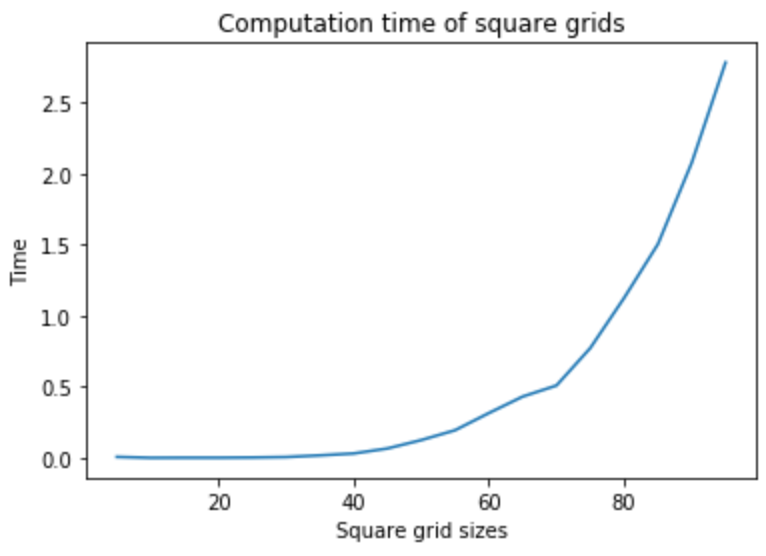
\includegraphics[width=0.6\linewidth]{Materials/runtime}
	\caption{Graph of how long it takes to solve the linear system vs. size of a square grid.}
	\label{runtime}
\end{figure}

	
\end{document}
\endinput
